In general simple linear regression is written as:\encV{$Y\approx
\beta_{0}+\beta_{1}X$}.\\We might read ``$\approx$'' as ``is 
approximately modeled as''

\paragraph{Estimating the Coefficients}
Let $\left\{ \left( x_{i},y_{i} \right) \right\}_{1\leq i\leq n}$
represent $n$ observations, our goal is to obtain coefficient estimates
$\widehat{\beta}_{0},\widehat{\beta}_{1}$ such that the linear model
fits the available data well, so that $y_{i}\approx\beta_{0}+\beta_{1}
x_{i}$ for $i\in\inter{1}{n}$, in other words we want an \emph{
intercept} $\beta_{0}$ and a \emph{slope} $\beta_{1}$\\For $i\in\inter{1
}{n}, e_{i}=y_{i}-\widehat{y}_{i}$ represents the $i^{th}$ \emph{
residual}\\
Then we define the \begin{center}\enc{$\text{RSS(\tR{Residual Sum of
Squares})}=\su{{i=1}}{n}e_{i}^{2}=\su{{i=1}}{n}\left( y_{i}- \widehat{
\beta_{0}}-\widehat{\beta_{1}}x_{i}\right)^{2}$}\end{center}.Using some calculus show 
that minimizers are \enc{$\begin{cases}\widehat{\beta_{1}}=\dfrac{\su{{
i=1}}{n}(x_{i}-\overline{x})(y_{i}-\overline{y})}{\su{{i=1}}{n}(x_{i}-
\overline{x})^{2}}\\\widehat{\beta}_{0}=\overline{y}-\widehat{\beta}_{1
}\overline{x}\end{cases}$}
\begin{figure}[H]
  \centering
  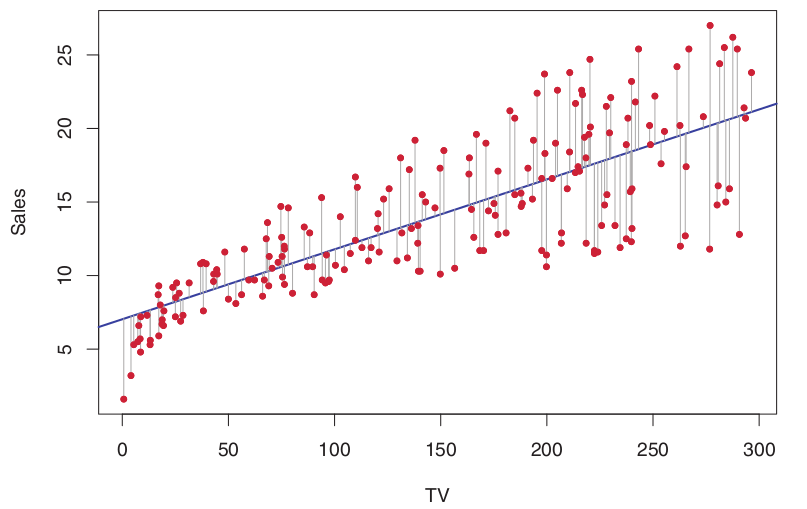
\includegraphics[width=.3\textwidth]{./chap/1chap/2sec/1images/1_leastSquares.png}
  \caption{The least squares fit for the regression of sales onto TV.}
  \label{fig:2.1}
\end{figure}
We can see on the following plots, that $\widehat{\beta}_{0},\widehat{\beta}_{1}$ minimize the RSS.
\begin{figure}[H]
  \centering
  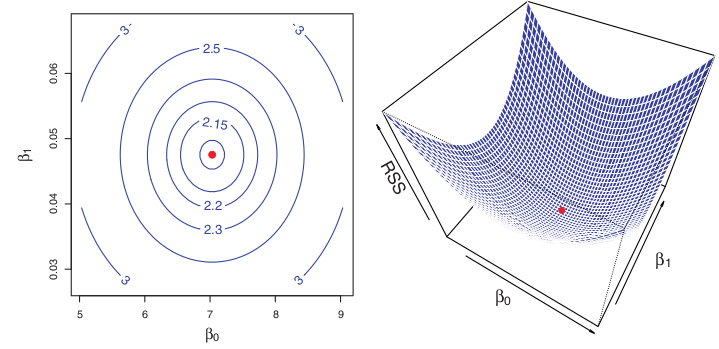
\includegraphics[width=.5\textwidth]{./chap/1chap/2sec/1images/2_leastSquaresCoefficients.png}
  \caption{Contour and 3-dimensionnal plots of the RSS on the 
Advertising data, using sales as the response and TV as the predictor}
  \label{fig:2.2}
\end{figure}

\paragraph{Assessing the Accuracy of the Coefficient Estimates}
When we assume that there is a relation between $X\text{ and }Y$ then
$Y=f\left( X \right)+\epsilon\begin{cases}f\text{ is a uknown function
 }\\\epsilon\text{ is a mean-zero random error term, is a catch-all for
what we miss with this simple model}\end{cases}$\\If $f$ is to be 
approximated by a linear function then we can write this relationship
as \encN{$Y=\beta_{0}+\beta_{1}X+\epsilon$}.\\This equation defines the
\emph{population regression line} which is the best approximation to
the true relationship between $X$ and $Y$.\\ We created $100$ random
$X_{s}$ and generated $100$ corresponding $Y_{s}$ from the model $Y=2+
3X+\epsilon$ where $\epsilon$ is generated from a normal distribution
with mean zero.
\begin{figure}[H]
  \centering
  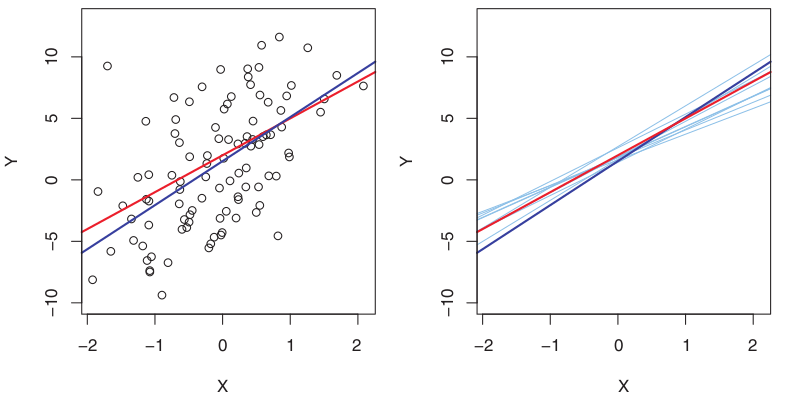
\includegraphics[width=\textwidth]{./chap/1chap/2sec/1images/3_leastSquaredErrorLineVsPopulationRegressionLine.png}
  \caption{The left-hand pannel:red line is the popuation regression
  line, and in blue line the least squares estimate for $f(X)$ bassed
  on the observed data, shown in black.\\The right-hand pannel: is the
  same graph that left-hand pannel but with 10 other least sqaures
  estimates with each a distinct training data set but from the same
  model}
  \label{fig:2.3}
\end{figure}
If we use the sample mean $
\widehat{\mu}$ to estimate $\mu$ this estimate is \emph{unbiased}, in
the sense that on average, we expect $\widehat{\mu}$ to equal $\mu$\\
We have etablished that the average $\widehat{\mu}$'s over many data
sets will be very close to $\mu$ but that a single estimate $\widehat{
\mu}$ may be a substantial underestimate or overestimate of $\mu$.
\tB{How far off will that single estimate of $\mu$ be? We generally 
answer to this question by computing the \emph{SE (Standard Error)} of
$\widehat{\mu}$ written as $SE(\widehat{\mu})$}:\begin{center}\enc{
$\V{\widehat{\mu}}=SE\left( \widehat{\mu} \right)^{2}=\dfrac{\sigma^{2}
}{n}$}\\$\sigma$ is the standard deviation of each of the realizations 
$y_{i}$ of $Y$.\end{center}
\begin{center}\enc{$
\begin{cases}SE\left(\widehat{\beta}_{0}\right)^{2}=\sigma^{2}\left[
\dfrac{1}{n}+\dfrac{\overline{x}^{2}}{\su{{i=1}}{n}\left(x_{i}-
\overline{x}\right)^{2}}\right]\\
SE\left(\widehat{\beta}_{1}\right)^{2}=
\dfrac{\sigma^{2}}{\su{{i=1}}{n}\left(x_{i}-\overline{x}
\right)^{2}}\end{cases}$}\\$\sigma^{2}=\V{\epsilon}$\end{center}\Moi{$SE\left(\widehat{\beta_{1}}
\right)$ is smaller when the $x_{i}$ are more spread out}For these
formulas we need to assume that the errors $\epsilon_{i}$ are
uncorrelated with $\sigma^{2}$. This is cleary not true but the formula
still turn out to be a good approximation.\\\sB{In general $\sigma$ is
unknown but can be estimated from the data, the estimate of $\sigma$ is
known as} \tR{\emph{Residual Standard Error}} \encB{$RSE=\sqrt{\dfrac{
RSS}{n-2}}$}.\\\Moi{Roughly speaking when $\sigma^{2}$ is estimated we
should write $\widehat{SE\left(\widehat{\beta_{1}}\right)}$}\\\\
Standard can be used to define \emph{confident interval}
\tR{For linear regression the $95\%$ confident intervals are} \begin{center}
\enc{$\begin{cases}\widehat{\beta_{0}}\pm 2\times SE\left(\widehat{
\beta_{0}}\right)\\\widehat{\beta_{1}}\pm 2\times SE\left(\widehat{
\beta_{1}}\right)\end{cases}$}\end{center}Standard error can be used
to perform hypothesis test, the most common test involves \emph{null
hypothesis} and \emph{alternative hypothesis}:\encB{$\begin{cases}
H_{0}:\beta_{1}=0\\H_{\alpha}:\beta_{1}\neq 0\end{cases}$}\\To test
null hypothesis we need to determine wehter $\widehat{\beta_{1}}$ is
sufficiently
far from zero that we can be confident that $\beta_{1}$ is non-null.\\
\emph{How far is far enough?} This depends on the $\widehat{\beta_{1}}$
accuracy then \\$\begin{cases}SE\left(\widehat{\beta_{1}}\right)\text{
is small, even relatively small values of }\widehat{\beta_{1}}\text{
can be a strong evidence that }\beta_{1}\neq 0\\SE\left(\widehat{
\beta_{1}}\right)\text{ is large then }\widehat{\beta_{1}}\text{ must 
be large in absolute value in order for us to reject }H_{0}\end{cases}$
\\In practice we compute a \emph{t-statistic} given by \begin{center}
\enc{$t=\dfrac{\widehat{\beta_{1}}-0}{SE\left(\widehat{\beta_{1}}
\right)}$}\\which measure the number of standard deviation that $
\widehat{\beta_{1}}$ is away from $0$.\end{center} \tB{If there is no
relationship between $X$ and $Y$ then we except that we will have a 
\emph{ t-distribution}}. It is a simple matter \tR{to observe the 
probability of observing any number equal to $|t|$ or larger in
absolute
value, \emph{assuming that }$\beta_{1}=0$} this probability is called
\tR{\emph{p-value}}.\\Roughly speaking a small \emph{p-value} indicates
that it is unlikely to observe such a substantial association between
the predictors and the response due to chance.\\\encN{Typical \emph{
p-value} cutoffs for rejecting $H_{0}$ is $5-1\%$}
\paragraph{Assessing the accuracy of the model}
Once we have rejected the null hypothesis in favor of the alternative
hypothesis it is natural to want to qualify to which the model fits the
data.
\subparagraph{Residual Standard Error} \tB{is an estimate of standard
deviation of $\epsilon$}, it means the average amount that the response
will deviate from the true regression line.
\subparagraph{$R^{2}$ statistic} it provides an alternative measure of
fit, and takes the form of a \emph{proportion} (the proportion of
variance explained). \tB{\emph{Total Sum of Squares}} \enc{$TSS=\su{{i=1}}{n
} \left(y_{i}-\overline{y}\right)^{2}$} represents the amount of 
variability
inherent to the response before the regression is performed, in 
contrast \emph{RSS measures the amount of variability that left
unexplained after performing regression}. \begin{center}\enc{$R^{2}=
	\dfrac{TSS-RSS}{TSS}$}\\Then $R^{2}$ measures the \emph{proportion of
variability in $Y$ that can be explained using $X$}\end{center}Recall
that \tR{correlation} defined as \begin{center}\enc{$\widehat{Cor(X,Y)}=
\dfrac{\su{ {i=1}}{n}\left(x_{i}-\overline{x}\right)\left(y_{i}-
\overline{y}\right)}{\sqrt{\su{ {i=1}}{n}\left(x_{i}-\overline{x}
\right)^{2}}\sqrt{\su{ {i=1}}{n}\left(y_{i}-\overline{y}\right)^{2}}}
$}\\$r=\widehat{Cor\left(X,Y\right)}$ is also a measure of the linear
relationship between $X$ and $Y$\end{center}\Moi{it can be shown that
in the simple regression setting $R^{2}=r^{2}$}
